\newcommand*{\figuretitle}[1]{%
    {\centering%   <--------  will only affect the title because of the grouping (by the
    \textbf{#1}%              braces before \centering and behind \medskip). If you remove
    \par\medskip}%            these braces the whole body of a {figure} env will be centered.
}

\section{Results}
\label{sec:validation}

Upon running our trained models on the dataset, we identified some classifiers that were doing
better than others in terms of successfully classifying genetic interactions as SL. This table
presents the top classifiers for each dataset that we tested. In every case, Random Forest was the
highest performing classifier. In general, it seems that using a random forest will correctly
estimate about 70\% of the SL gene interactions. 

An initial concern was that our model was over-fitting the tree due to the 100\%
classification accuracy on the training data. To check that we weren't over-fitting, we re-trained
the models with a smaller forest size to see if the training data accuracy would change. Our
results are presented in table \emph{X}. Despite changing our forest size, the model maintained an
accuracy of 100\% on the training data but with consistent drops in test data classification. From
these results, we came to the conclusion that using a tree size of 128 or 256 would be ideal since
it would maximize test data classification. Further research is necessary to determine if the
relationship between forest size and test accuracy is parabolic in nature or is upper bounded. 

\begin{figure}[t!]
\centering
%
\figuretitle{Classifer Results}
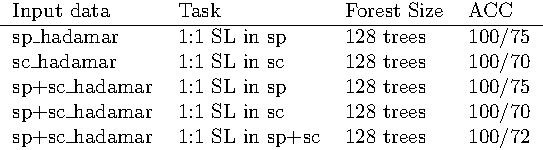
\includegraphics[width=.48\textwidth]{figs/best-class}
%
\end{figure}

% }}}

% Accuracy as a function of path length plots {{{

\begin{figure}[t!]
\centering
%
\figuretitle{Changing Forest Size}
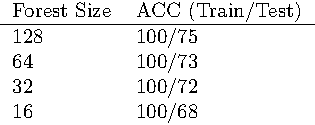
\includegraphics[width=.38\textwidth]{figs/forest-size}
%
\end{figure}

Given that the initial results were very promising, we took a closer look at the model for the Sp to
determine if the model could be reliable over a larger dataset. We ran a stratified 5 fold cross
validation instead of a normal 5-fold cross validation since we are dealing with classification and
want about an equal number of each type in each split. After running the model through validation,
we found that the model's accuracy was consistent around 75\% which is the same result we initially
received. This means that the model could be applied to other datasets and would be minimally
affected by bias. We would test this theory, but the lack of relevant data make testing across
two different datasets difficult. Furthermore, we were surprised to find that that even random
forests with smaller forest sizes yielded fairly consistent results when put through the same
stratified 5 fold cross validation. 

\begin{figure}[t!]
\centering
%
\figuretitle{Stratified 5 Fold for Size=128}
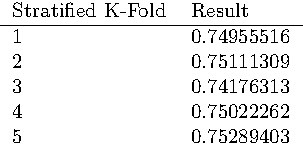
\includegraphics[width=.38\textwidth]{figs/strat-128-dim}
%
\end{figure}

% }}}

% Accuracy as a function of path length plots {{{

\begin{figure}[t!]
\centering
%
\figuretitle{Stratified 5 Fold}
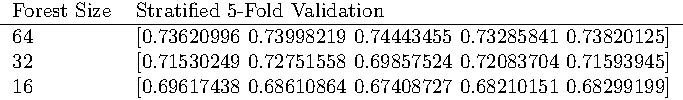
\includegraphics[width=.48\textwidth]{figs/strat}
%
\end{figure}

The PR curve of our model isn't ideal, but it shows that our model has promise and can be improved.
The baseline is 50\% and it appears that for about 50\% recall we can have 75\% precision which is
very reasonable. This could be further improved by trimming the feature set or playing around
with how different input vectors would change results. We firmly believe that our research shows that there is more work to be done studying how graph analysis tools like node2vec can be used to study genetic interactions. The area under our ROC curve is .75, which is a strong indicator that the random forest does a good job of differentiating the different classes. Something else we noticed was that the identification rate for both SL and non-SL were about the same which suggests that there might be value in trying to indentify non-SL interactions and assume interactions not classified are SL. Once again, this is an opportunity for further research. 

\begin{figure}[t!]
\centering
%
\figuretitle{ROC Curve}
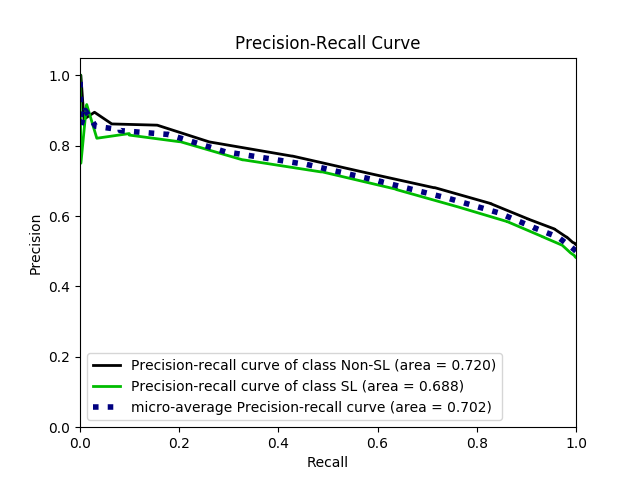
\includegraphics[width=.48\textwidth]{figs/pr-curve}
%
\end{figure}

% }}}

% Accuracy as a function of path length plots {{{

\begin{figure}[t!]
\centering
%
\figuretitle{PR Curve}
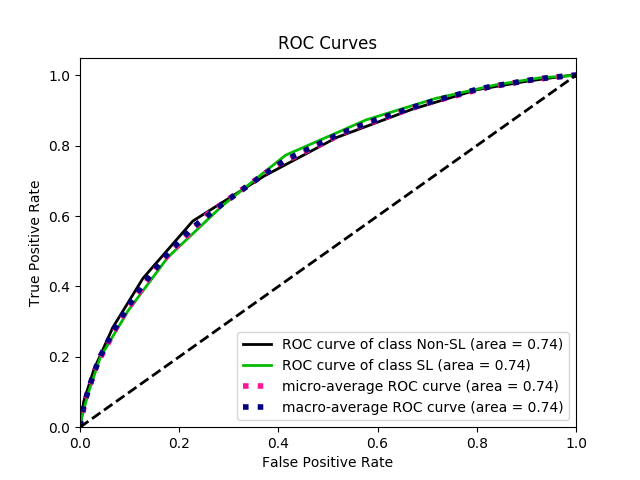
\includegraphics[width=.48\textwidth]{figs/testplot}
%
\end{figure}

